\chapter{Testing}
Testing is an important aspect of the work carried out in this thesis. In this chapter the
test setup are described. How the tests are carried out, some of the results and some
imidiate results.


\section{Test Environment}
The test environment are two connected pipe segments. A Y-junction and an L-bend. This
pipe segments are connected, according to Figure \ref{chap7:fig-environment}.

\begin{figure}[htbp]
    \centering
    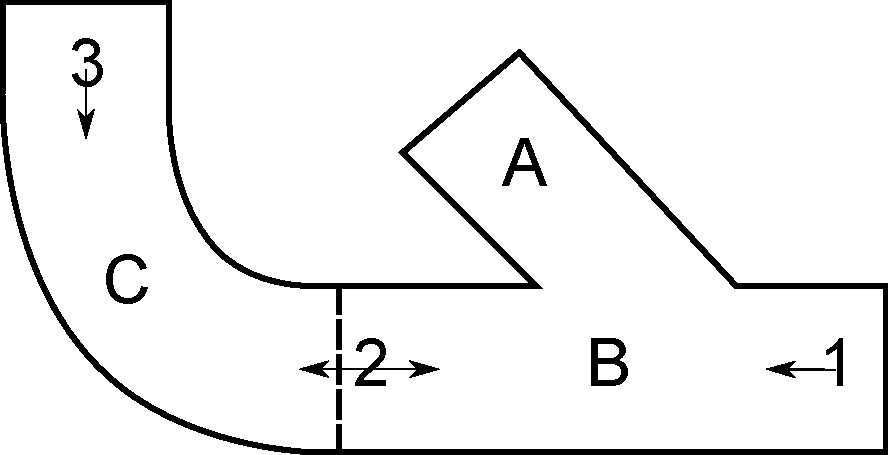
\includegraphics[width=0.7\textwidth]{pics/test-environment}
    \caption{The test environment}
    \label{chap7:fig-environment}
\end{figure}

There are six points of interest in this environment. 
The numbers 1-3 are the places where the sensors will be put and record snapshots of the pipe. 
The letters A-C are places where irregularities and anomalies in the pipes are placed. 

This places are all described in detail in the next section.


\section{Test Cases}
To test the performance and robustness of the developed algorithms three cases are used,
ideal situation, situation with obstacles with regular surface, and obstacles where the
surface are irregular. This cases are carried out for all the 3 different places described
in the previous section.

\subsection{Control Case}


\subsection{Irregular surfaced anomalies}


\subsection{Regular surfaced anomalies}



\section{Test Results}


